\chapter{Results}
\label{chap:results}

\section{From a kitchen benchmark to a controlled task}
\label{sec:results-journey}
The project began as a study of whether deployable models could perform the
RoboCasa kitchen benchmark \parencite{nasiriany2024robocasa}, whose reference
policy is a large foundation model (GR00T~N1.6, \cite{nvidia2025gr00t}). GR00T is
powerful --- it reached approximately 54\% zero-shot on the tested tasks --- but at
several billion parameters it cannot be fine-tuned or deployed within a 12~GB GPU.
Two deployable small models (SmolVLA and ACT) were therefore fine-tuned on RoboCasa
demonstrations and evaluated on the same kitchen ``pick from the counter and place in
the cabinet'' tasks. Both completed \emph{zero} of twenty trials each: the cluttered
kitchen benchmark was out of reach for small models even after task-specific
fine-tuning. A third candidate, $\pi_0$, could not be brought up in this environment
--- training aborted before the first optimisation step owing to an incompatibility
between the installed \texttt{transformers} release and the PaliGemma backbone
expected by the policy implementation --- so no $\pi_0$ result is reported here.

Note that the GR00T figure quoted above is a zero-shot result, whereas SmolVLA and ACT
were fine-tuned; the comparison is therefore conservative with respect to the small
models, and \reffig{fig:journey} should be read with that asymmetry in mind.

The evaluations used the same closed-loop protocol described in
\refsec{sec:m-eval}: twenty language-conditioned episodes per policy, each a distinct
kitchen ``pick from the counter and place in the cabinet'' instruction with a fresh
seed. The zero success rate was not a marginal miss but a categorical one --- the
small policies did not reliably grasp the varied kitchen objects in the cluttered
scenes, let alone place them --- which is why simply collecting more data or tuning
hyper-parameters was judged unlikely to help within the available budget.

This negative result motivated the strategy adopted for the rest of the thesis:
step back to a simpler, controlled task, get the methodology right, and then scale
the lessons up. The intermediate UR10e pilot deliberately reduced every difficulty
that RoboCasa compounds at once: a single rigid object rather than a diverse
inventory, a fixed base, a small set of known positions, and an uncluttered
tabletop. Under those conditions the same small models that failed RoboCasa learned
the task, confirming that the earlier failure was one of task and data difficulty
rather than of the models being fundamentally incapable. The three methodological
lessons carried forward --- a verified success metric, varied demonstrations, and a
memory-feasible training configuration --- are exactly the ingredients that the
supermarket system in the remainder of this chapter builds upon. An intermediate pilot on a fixed-base UR10e cube pick-and-place ---
comparing ACT and SmolVLA over five cube positions --- confirmed that small models
\emph{can} learn a controlled task, reaching approximately 47\% (ACT) and 53\%
(SmolVLA) placement. The two policies failed in different places rather than sharing
weaknesses: the from-scratch ACT baseline never grasped at the two positions requiring
the largest joint-space swing, whereas SmolVLA grasped at every position but placed
unreliably at one, and both struggled most at the position combining the longest reach
with the largest swing to the basket. That the VLA and the non-VLA baseline fail
differently is itself informative --- it indicates that the pretrained
vision--language prior changes \emph{which} part of the task is hard, not merely how
often it succeeds --- and it foreshadows the grasp-versus-place decomposition seen in
the supermarket results (\refsec{sec:results-peritem}). That pilot also surfaced three methodological lessons that
proved decisive: a success-metric bug had inflated a real 40\% to a reported 80\%;
duplicated demonstrations provided no variety to learn from; and fully unfreezing
the vision encoder exceeded the memory budget. Fixing the metric and the data
mattered more than the model choice. \reffig{fig:journey} summarises this
progression, and \reffig{fig:robots} shows the three robots involved.

\begin{figure}[ht]
\begin{center}
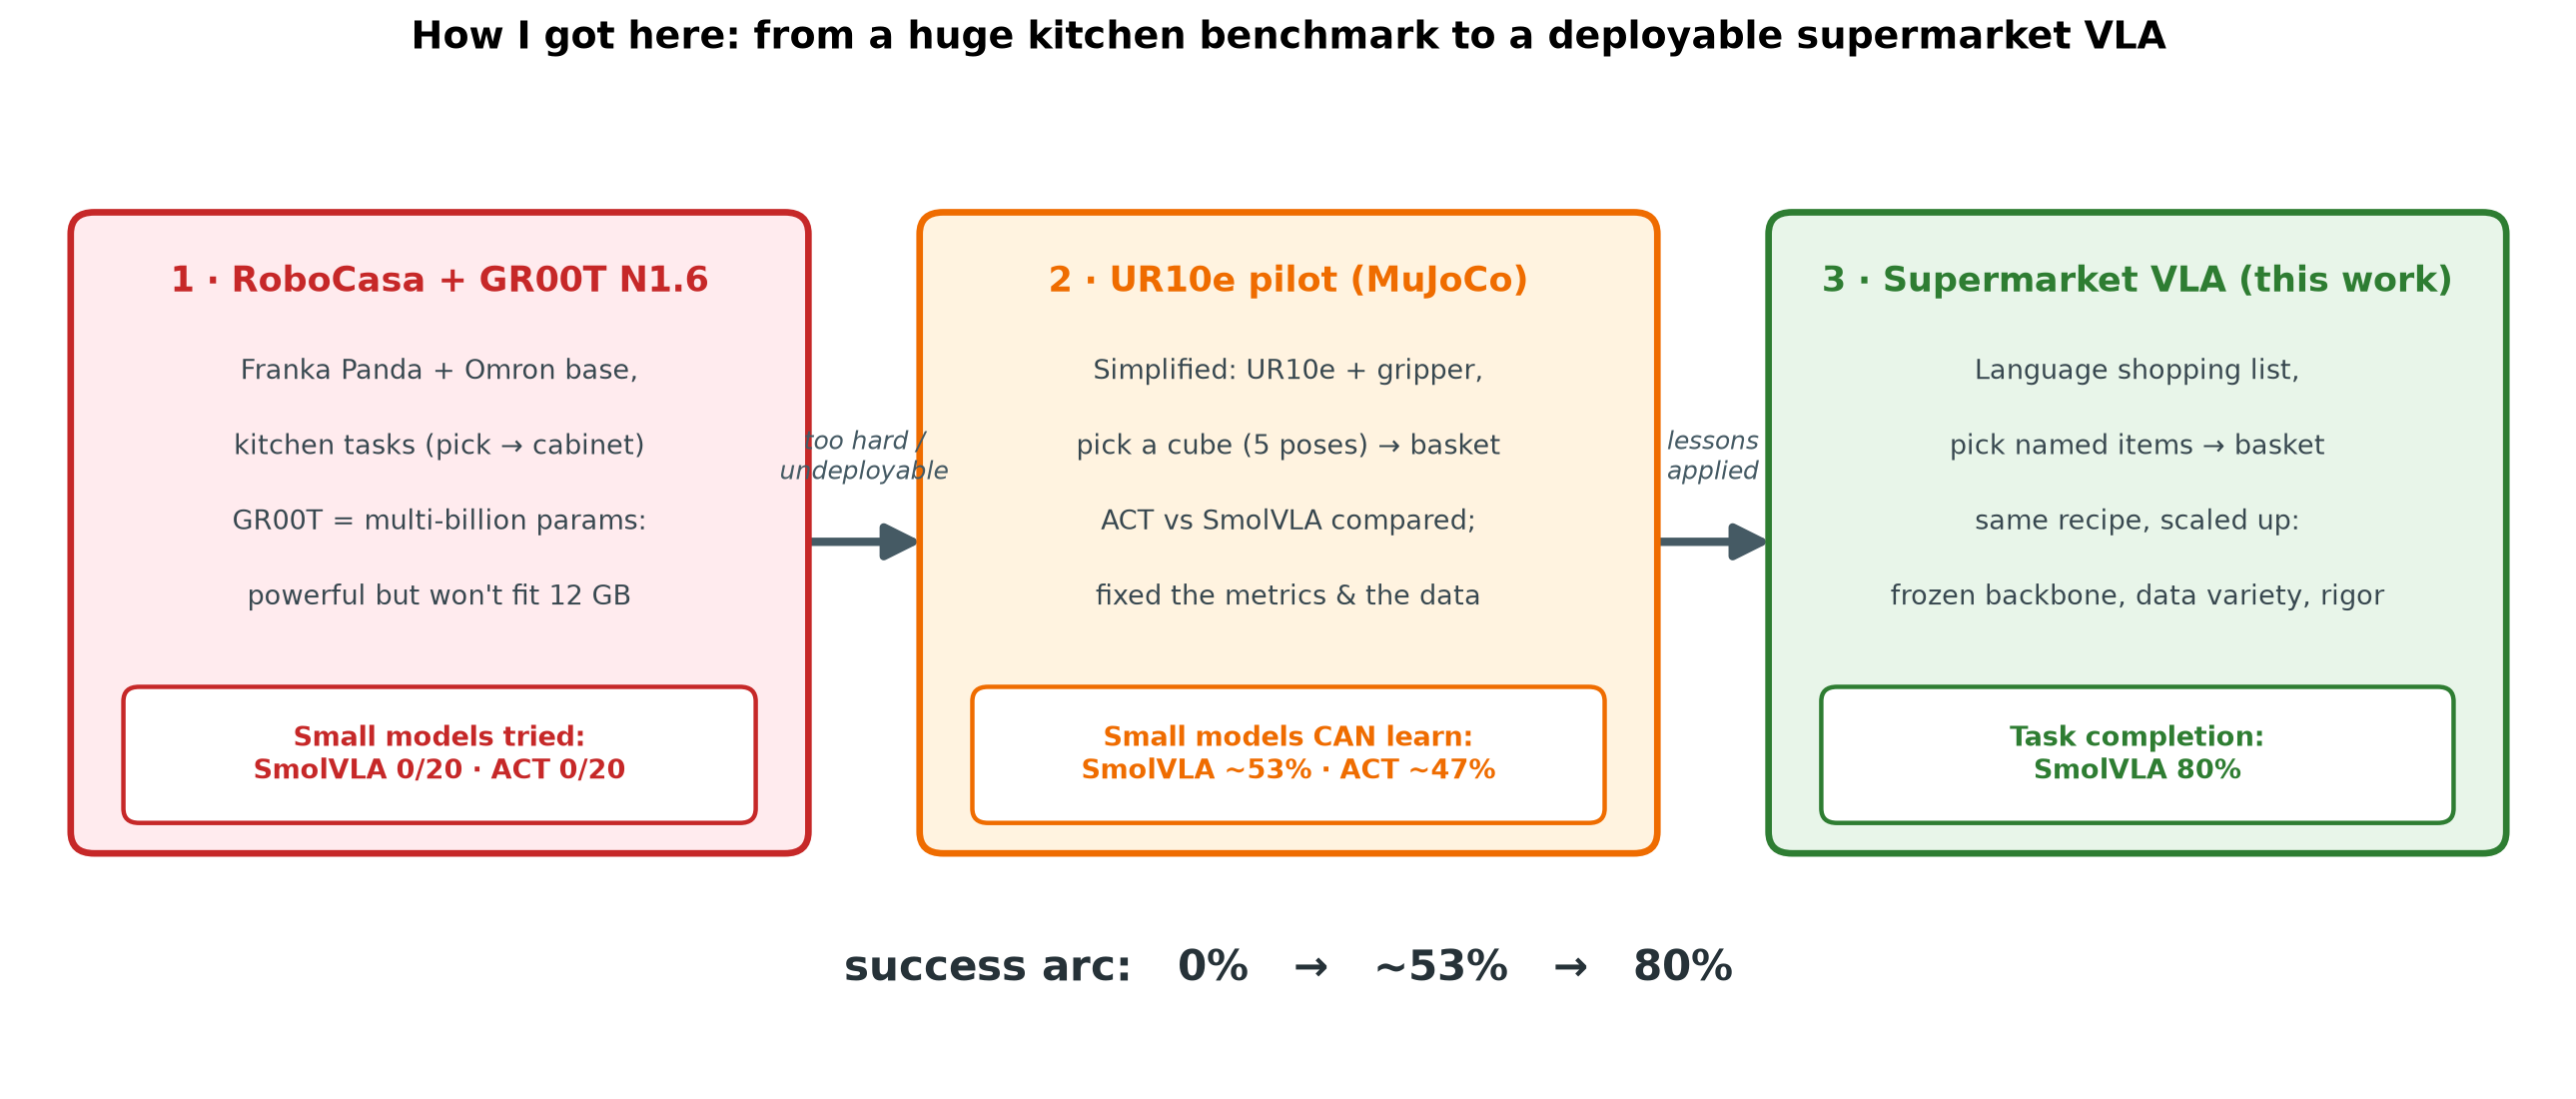
\includegraphics[width=\textwidth,
    alt={A three-stage progression diagram: RoboCasa with GR00T (small models 0 percent), the UR10e pilot (about 53 percent), and the supermarket VLA (80 percent), linked by arrows.}]{figures/journey_prior_work}
\end{center}
\caption{The progression of the project: a large model works on RoboCasa but is
undeployable; small models fail the benchmark; a controlled UR10e pilot succeeds;
the lessons scale to the supermarket task. Success rate rises 0\% $\rightarrow$
$\sim$53\% $\rightarrow$ 80\%.}
\label{fig:journey}
\end{figure}

\begin{figure}[ht]
\begin{center}
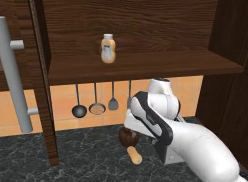
\includegraphics[width=0.32\textwidth,
    alt={The RoboCasa Franka robot doing a kitchen task.}]{figures/prog_robocasa}\hfill
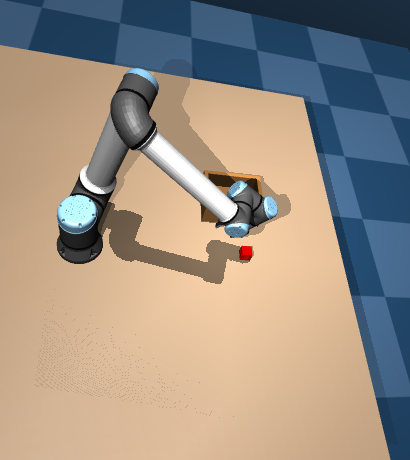
\includegraphics[width=0.32\textwidth,
    alt={The UR10e arm picking a cube on a table in the pilot study.}]{figures/prog_ur10e}\hfill
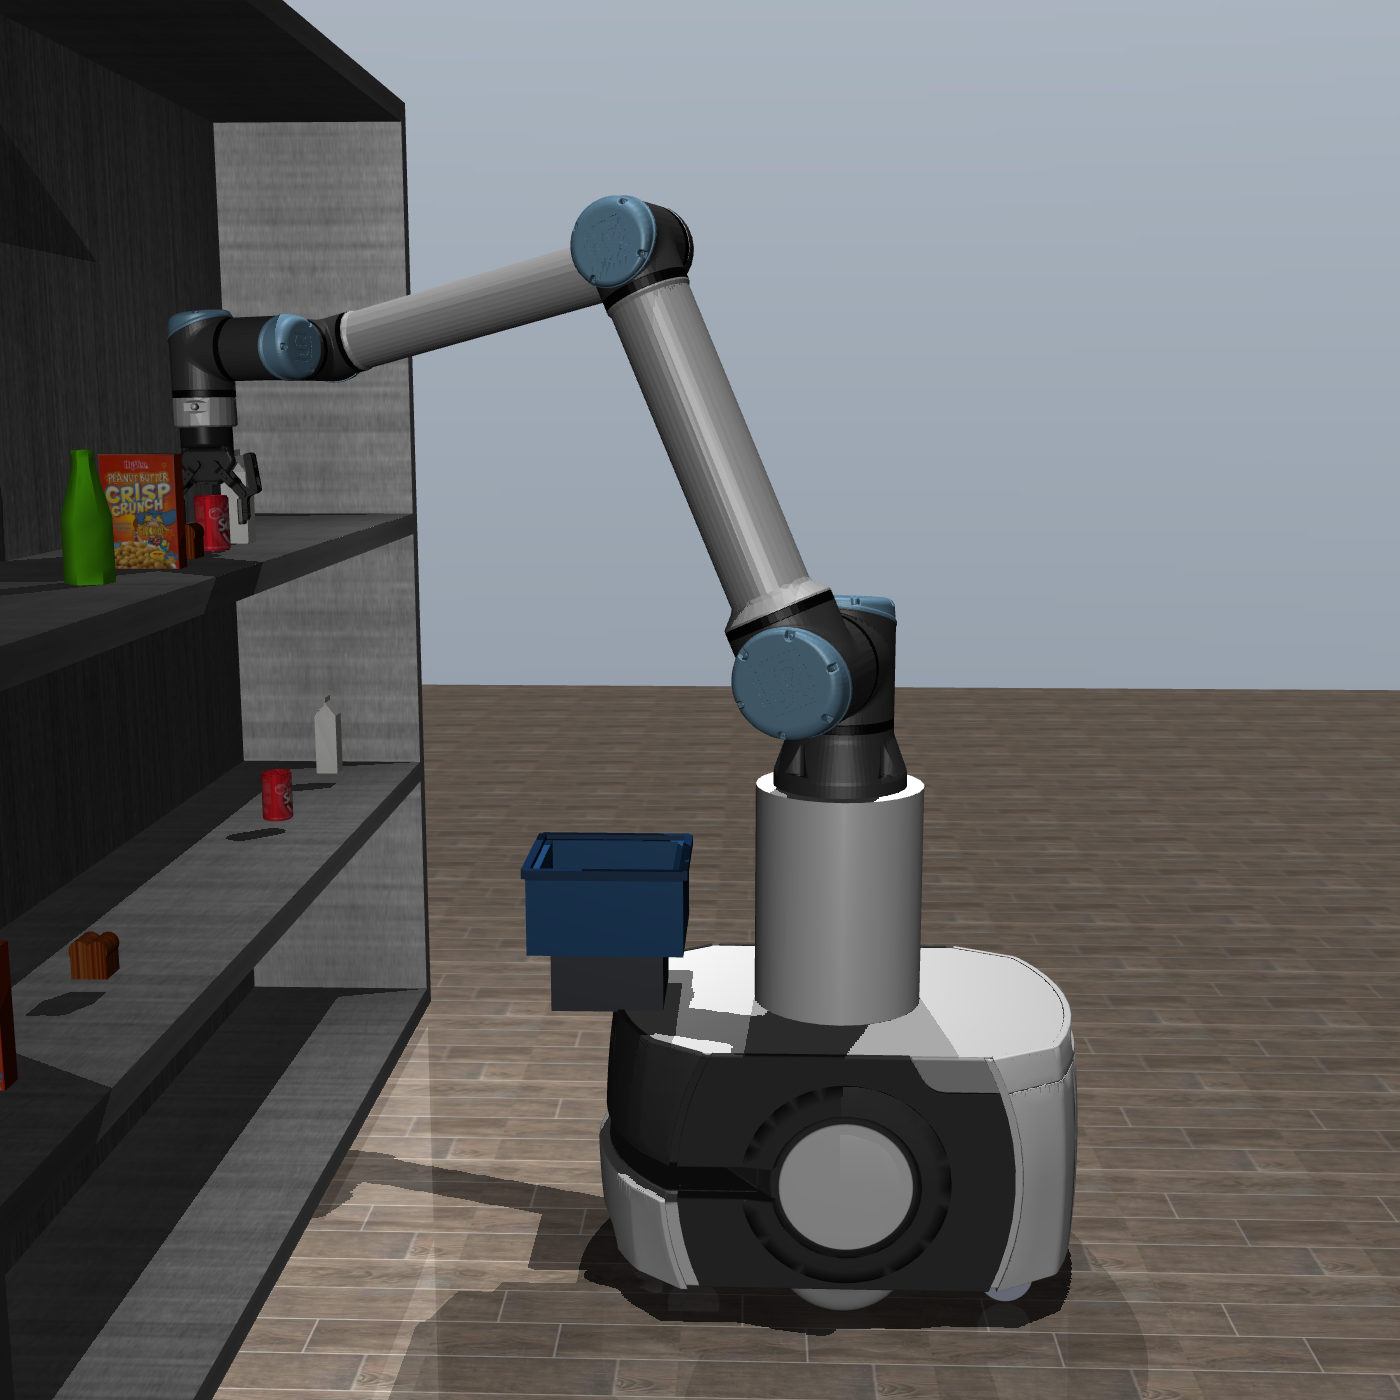
\includegraphics[width=0.32\textwidth,
    alt={The supermarket mobile manipulator at the shelf.}]{figures/prog_supermarket}
\end{center}
\caption{The three robots, left to right: RoboCasa (Franka on a mobile base,
GR00T~N1.6); the fixed-base UR10e pilot; and the supermarket mobile manipulator
studied in this thesis.}
\label{fig:robots}
\end{figure}

\section{Headline result}
\label{sec:results-headline}
On the supermarket task, the fine-tuned SmolVLA policy (best checkpoint; see
\refsec{sec:results-checkpoint}) achieves an \textbf{80\% task-completion rate}
(95\% Wilson CI 70--87) and a \textbf{92.5\% grasp success rate}, measured over
\textbf{320 closed-loop trials} (four items, 20 trials each, across four
checkpoints; the best-checkpoint headline aggregates its 80 item-trials with the
per-item detail below). The result is not a single fortunate demonstration but an
aggregate over many trials with confidence intervals throughout.

This figure should be read against two reference points. Kiviranta reports an 80\%
single-task success rate fine-tuning the same SmolVLA checkpoint on real SO-101
hardware from around 100 demonstrations \cite{kiviranta2025smolvla}, so the result
here is in the same regime as an independent study on real hardware, obtained under a
strict 12~GB budget and with a language-conditioned choice among four items rather
than a single fixed task. The second reference point is internal: the same family of
small models scored 0/20 on the RoboCasa benchmark (\refsec{sec:results-journey}), so
the 80\% here reflects not a change of model but the controlled task and the
disciplined methodology built around it. Together these answer RQ1 affirmatively --- a
compact VLA is deployable on a single consumer GPU at a useful success rate --- while
the remainder of the chapter examines \emph{why} it works and where it does not.

\section{Per-item results}
\label{sec:results-peritem}
\reftab{tab:peritem} and \reffig{fig:peritem} give the per-item breakdown for the
selected checkpoint. Three of the four items complete at or above 75\%, and two at
or above 90\%; grasping is essentially solved for three items at 100\%. The milk
carton is the weakest item, which is analysed in \refsec{sec:disc-limits}.

\begin{table}[ht]
\caption{Per-item grasp and task-completion (placement) rates for the selected
checkpoint, with $n=20$ trials per item and Wilson 95\% confidence intervals on the
placement rate.}
\begin{center}
\tagpdfsetup{table/header-rows={1}}
\begin{tabular}{lccc}
\toprule
Item & Grasp & Placed (task complete) & 95\% CI \\
\midrule
Cola can      & 100\% & 95\% & 76--99 \\
Water bottle  & 100\% & 90\% & 70--97 \\
Bread loaf    & 100\% & 75\% & 53--89 \\
Milk carton   & 70\%  & 60\% & 39--78 \\
\midrule
Overall       & 92.5\% & 80\% & 70--87 \\
\bottomrule
\end{tabular}
\end{center}
\label{tab:peritem}
\end{table}

\begin{figure}[ht]
\begin{center}
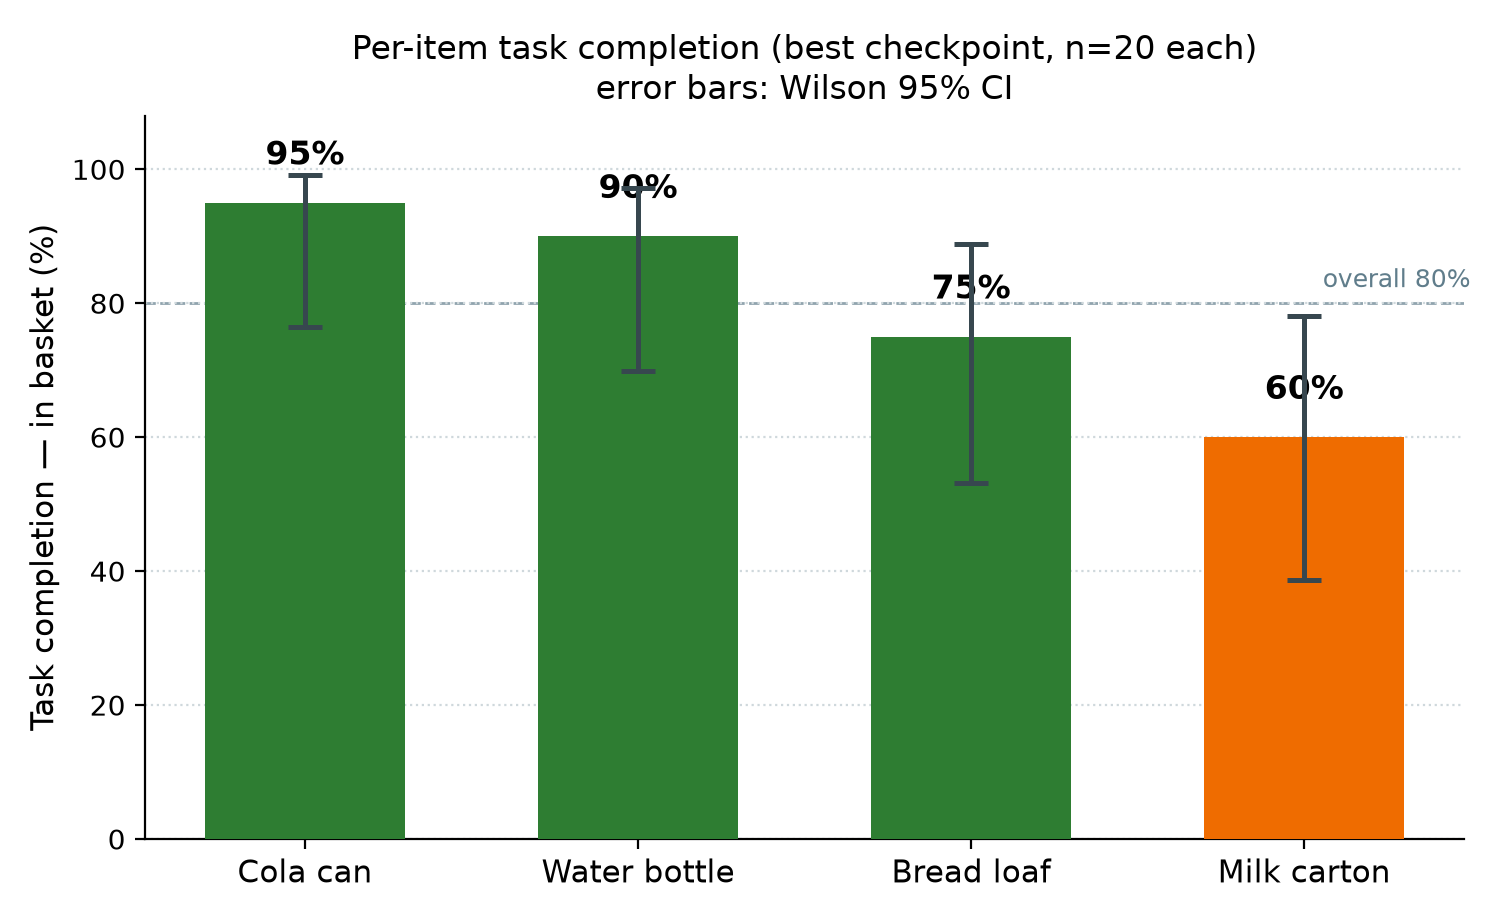
\includegraphics[width=0.8\textwidth,
    alt={A bar chart of per-item task-completion rates with Wilson confidence-interval error bars: cola 95 percent, water bottle 90 percent, bread 75 percent, milk 60 percent.}]{figures/per_item_success}
\end{center}
\caption{Per-item task-completion rate for the selected checkpoint, with Wilson
95\% confidence-interval error bars ($n=20$ each). The dashed line marks the 80\%
overall rate.}
\label{fig:peritem}
\end{figure}

The per-item pattern is informative. The \textbf{cola can} and \textbf{water
bottle} are the strongest items (95\% and 90\% placement, both 100\% grasp): the can
is compact and easy to grip, and the bottle, although tall, sits at the near-side
reach where the wrist camera has a clean view during the descent, and its higher grip
point (\refsec{sec:m-grasp}) gives a stable hold. The \textbf{bread loaf} grasps
perfectly (100\%) but places slightly less reliably (75\%), consistent with its
larger footprint making the final drop into the tote more sensitive to lateral
error. The \textbf{milk carton} is the clear outlier (70\% grasp, 60\% placement).
Its weakness has two causes, neither of them kinematic reach. First, it is the tallest
item on the shelf, so its peak lift clears the \SI{0.05}{m} grasp threshold by the
smallest margin of any item (median \SI{0.054}{m}); the grasp metric is therefore
least reliable precisely for this item, and its 70\% figure is better read as a lower
bound than as a measurement. Second, the learned reach exhibits a consistent inward
bias: all four items are approached slightly short of their true lateral position,
toward the shelf centre, so the items furthest from the centre are approached least
accurately. Note that the milk carton is \emph{not} the most extended target --- the
water bottle sits \SI{8}{cm} further from the centreline (\refsec{sec:m-env}) and
achieves 100\% grasp --- and the scripted expert reaches 98\% on the carton with no
item-specific tuning, so the difficulty lies in the learned policy rather than in the
robot's kinematics. That the
milk carton placed more reliably at earlier checkpoints (\refsec{sec:results-checkpoint})
indicates the weakness is not intrinsic to the item but an artefact of where in
training the deployed checkpoint was taken, and is therefore recoverable
(\refsec{sec:disc-limits}). The overall separation between a near-solved grasp phase
and a more variable placement phase --- 92.5\% versus 80\% --- localises the residual
difficulty to the final drop rather than to perception or reaching, a theme returned
to in the failure analysis below.

\section{Failure analysis: from 0\% to 80\%}
\label{sec:results-diagnosis}
The first policy trained on the supermarket task placed items \emph{0\%} of the
time (0 of 12 trials; grasp 9 of 12). That baseline rests on a much smaller sample
than the 80 trials per checkpoint reported above --- a 0/12 result carries a Wilson
95\% confidence interval of roughly 0--24\% --- so the comparison with the final
figure should be read as an order-of-magnitude improvement rather than an exact
80-point gain. Rather than assume a broken policy, a single episode was traced in
detail.
The policy in fact performed the whole task --- grasping the item, carrying it, and
lowering it to within about two centimetres of the basket --- before (a) releasing
about ten centimetres short, so the item rolled out of the small basket, and
(b) failing to stop cleanly, swinging back toward the shelf and occasionally
knocking the item out. The failure was therefore one of \emph{final-drop precision
and observability}, not of task understanding: perception, language, grasping and
transport all worked. \reffig{fig:nearmiss} depicts this failure mode
schematically.

\begin{figure}[ht]
\begin{center}
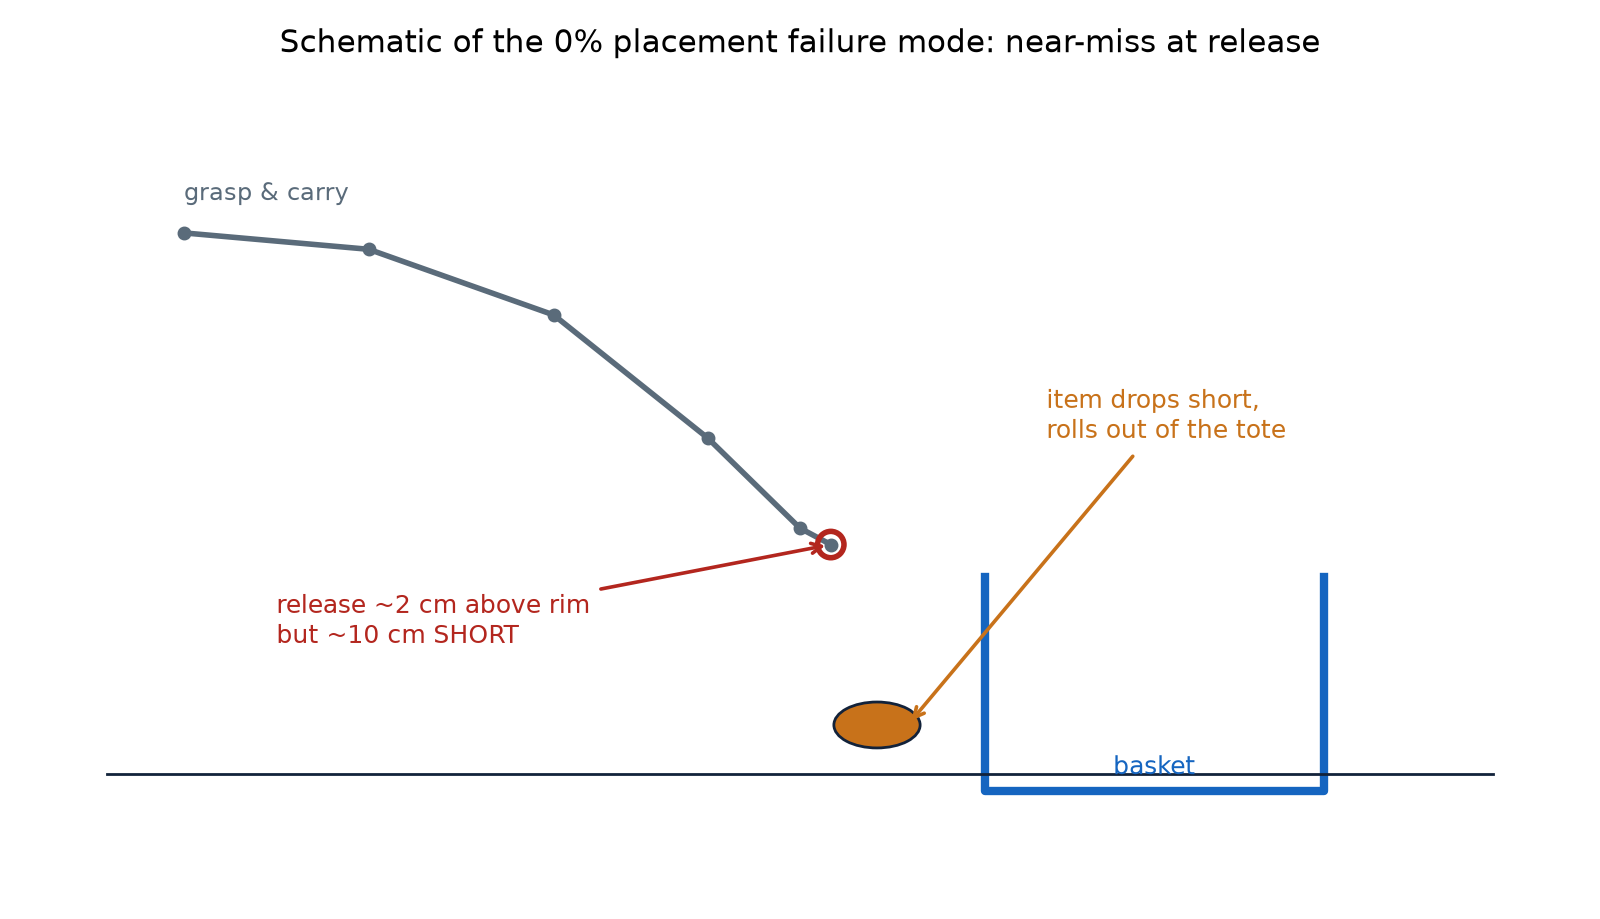
\includegraphics[width=0.8\textwidth,
    alt={A side-view schematic of the near-miss failure: the gripper carries and lowers the item but releases about ten centimetres short of the basket, so the item drops short and rolls out.}]{figures/fig_nearmiss}
\end{center}
\caption{Schematic of the initial 0\% placement failure. The policy grasps,
carries and lowers the item to just above the rim height, but releases
approximately ten centimetres short of the basket, so the item drops outside the
tote and rolls away --- a near-miss, not a failure of task understanding.}
\label{fig:nearmiss}
\end{figure}

This diagnosis pointed to three targeted changes, none of which involved scaling
the model: (i) \emph{clean episode boundaries} in the demonstrations, ending each
demo at placement so the policy is not taught to move away after releasing;
(ii) a \emph{dedicated basket camera} (\reffig{fig:basketcam}), because the policy
could previously barely see the drop target; and (iii) a \emph{wider basket} that
tolerates the residual near-miss. Together these raised placement from 0\% to 80\%.

Each fix targets a distinct facet of the diagnosis. The \emph{clean episode
boundary} is a data correction: by ending every demonstration at the moment of
placement, the policy is no longer shown the return-to-home motion and therefore does
not learn to move away immediately after releasing, which had been re-opening the
grip near the shelf and dislodging the item. The \emph{basket camera} is an
observability correction: previously the tote was visible only obliquely and late,
through the wrist and scene views, so the policy had little signal with which to
judge the final centimetres of the descent; a dedicated view of the drop target
supplies exactly that signal throughout the carry and release. The \emph{wider tote}
is a tolerance correction: it enlarges the target footprint so that the residual
lateral error at release --- which the other two fixes reduce but do not eliminate ---
still lands the item inside. It is worth emphasising that none of these changes
increases the model's capacity; the gain comes entirely from what the policy is
taught, what it can see, and how forgiving the target is. This is the central answer
to RQ4: the initial failure was a specific, localisable defect at the end of the
motion, and it was corrected by diagnosis rather than by scale.

\begin{figure}[ht]
\begin{center}
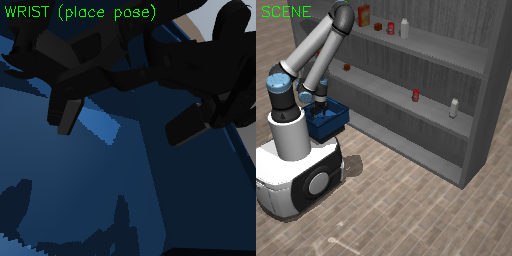
\includegraphics[width=0.49\textwidth,
    alt={The basket seen poorly from the wrist camera before the fix.}]{figures/basket_visibility}\hfill
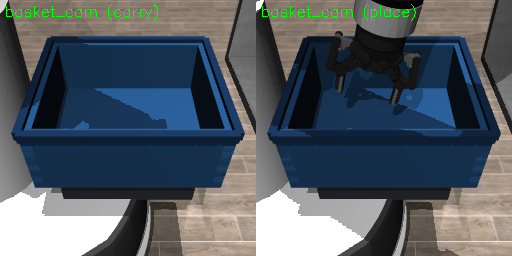
\includegraphics[width=0.49\textwidth,
    alt={The dedicated basket camera providing a clear view of the tote and the gripper descending into it.}]{figures/basket_cam}
\end{center}
\caption{Motivation and fix for the placement failure. Left: the basket is poorly
visible from the existing views. Right: the added basket camera gives a clear view
of the drop target throughout the carry and release.}
\label{fig:basketcam}
\end{figure}

\section{Language grounding}
\label{sec:results-language}
To test whether the policy genuinely uses the instruction rather than executing a
fixed motion, the scene was held constant and only the instruction word was
changed. \reftab{tab:grounding} reports the gripper's lateral ($y$) position at
the reach, against the target item's true position. The arm reaches the
\emph{named} item --- left for milk, centre for bread, right for the water bottle
--- so the target moves with the word. This is genuine language grounding, not a
memorised trajectory; the graded per-item success rates in
\reftab{tab:peritem} are likewise the signature of a learned controller rather than
a lookup.

The design of this test is deliberately adversarial to the null hypothesis. If the
policy had learned a single fixed reaching motion --- ignoring the instruction and
exploiting, say, the most salient object --- then changing only the words would leave
the reach unchanged, and the reached position would be constant across the three
instructions. Instead the reached lateral position tracks the named item across the
full width of the shelf, from $-0.24$ to $+0.29$\,\si{m}, a span far larger than the
few-centimetre residual error, so the instruction is demonstrably the causal variable.
This matters because language conditioning is the property that distinguishes a VLA
from the non-VLA ACT baseline (\refsec{sec:bg-act}) and is, per
\textcite{kiviranta2025smolvla}, easy to claim but fragile in practice; verifying it
with a controlled intervention rather than assuming it is therefore central to
answering RQ3. The small systematic undershoot on the far item (reaching $+0.29$ for a
target at $+0.34$) belongs to the \emph{water bottle}, not the milk carton, which sits
at $-0.26$. It is not specific to that item: all four items are reached slightly short
of their true lateral position, a consistent inward bias toward the shelf centre. Such
a bias is characteristic of a policy interpolating between demonstrated trajectories
rather than localising each item independently, and reflects reduced precision at the
extremes of the demonstrated range rather than a failure of grounding.

\begin{table}[ht]
\caption{Language-grounding test. With the scene fixed and only the instruction
changed, the gripper reaches the named item's lateral position.}
\begin{center}
\tagpdfsetup{table/header-rows={1}}
\begin{tabular}{lcc}
\toprule
Instruction & Item's $y$ (m) & Gripper reached $y$ (m) \\
\midrule
``milk carton''  & $-0.26$ & $-0.24$ \\
``loaf of bread'' & $\phantom{-}0.00$ & $-0.01$ \\
``water bottle'' & $\phantom{-}0.34$ & $\phantom{-}0.29$ \\
\bottomrule
\end{tabular}
\end{center}
\label{tab:grounding}
\end{table}

\section{Checkpoint selection}
\label{sec:results-checkpoint}
\reftab{tab:checkpoints} and \reffig{fig:checkpoints} report the closed-loop
performance of all four saved snapshots, evaluated over 80 trials each. The
15{,}000-step checkpoint attains the highest task-completion rate at 80\%, and was
the one deployed.

The differences between checkpoints must, however, be interpreted with care. Because
every checkpoint was evaluated on the same trial seeds, the trials are paired and
McNemar's exact test applies. Applied to task completion, \emph{no} pair of
checkpoints differs significantly (all $p \ge 0.19$ uncorrected, and all $p = 1.00$
after Holm correction for the six pairwise comparisons). On the grasp sub-task the
picture is different: grasp success at 15k is significantly better than at 5k
($p = 0.008$; Holm-corrected $p = 0.048$), while the remaining comparisons do not
survive correction. The defensible conclusion is therefore narrow: training beyond
5{,}000 steps measurably improves \emph{grasping}, but the four checkpoints are
statistically indistinguishable on end-to-end task completion at $n=80$. The apparent
\SI{5}{\percent} dip from 15k to 20k is within sampling noise and should not be read
as over-training; a per-item breakdown (\reftab{tab:peritemckpt}) shows it is driven
almost entirely by a single item, the water bottle, rather than being a consistent
regression.

A further consideration is that the learning-rate schedule was configured for
30{,}000 decay steps but training was stopped at 20{,}000
(Appendix~\ref{app:Implementation}), so the cosine decay was truncated at roughly two-thirds
of its intended course and the learning rate at 15k was still $1.68\times10^{-5}$,
about 17\% of peak. None of the checkpoints represents a converged endpoint.

The methodological point stands independently of the ranking, and is what matters for
RQ2: closed-loop task success and the training objective are not monotonically
related, so the decision of which snapshot to deploy must be made on measured
behaviour rather than on the training signal. Here that choice was consequential only
in the weak sense that the final checkpoint was not the empirical best.

\begin{table}[ht]
\caption{Overall task-completion rate by training checkpoint ($n=80$ each), with
Wilson 95\% confidence intervals. The 15k checkpoint is selected.}
\begin{center}
\tagpdfsetup{table/header-rows={1}}
\begin{tabular}{lcc}
\toprule
Checkpoint (steps) & Task completion & 95\% CI \\
\midrule
5{,}000  & 68.8\% & 58--78 \\
10{,}000 & 68.8\% & 58--78 \\
\textbf{15{,}000} & \textbf{80.0\%} & \textbf{70--87} \\
20{,}000 & 75.0\% & 65--83 \\
\bottomrule
\end{tabular}
\end{center}
\label{tab:checkpoints}
\end{table}

\begin{table}[ht]
\caption{Placement success per item and per checkpoint ($n=20$ per cell). The
\SI{5}{\percent} aggregate drop from 15k to 20k is not consistent across items: the
milk carton improves by four trials and the bread loaf is unchanged, while the water
bottle accounts for the entire decline.}
\begin{center}
\tagpdfsetup{table/header-rows={1}}
\begin{tabular}{lccccc}
\toprule
Checkpoint & Cola can & Water bottle & Milk carton & Bread loaf & Overall \\
\midrule
5{,}000  & 90\% & 50\% & 85\%  & 50\% & 68.8\% \\
10{,}000 & 95\% & 30\% & 100\% & 50\% & 68.8\% \\
\textbf{15{,}000} & 95\% & 90\% & 60\% & 75\% & \textbf{80.0\%} \\
20{,}000 & 90\% & 55\% & 80\%  & 75\% & 75.0\% \\
\midrule
Change 15k$\rightarrow$20k & $-1$ & $\mathbf{-7}$ & $+4$ & $0$ & $-4$ \\
\bottomrule
\end{tabular}
\end{center}
\label{tab:peritemckpt}
\end{table}

\begin{figure}[ht]
\begin{center}
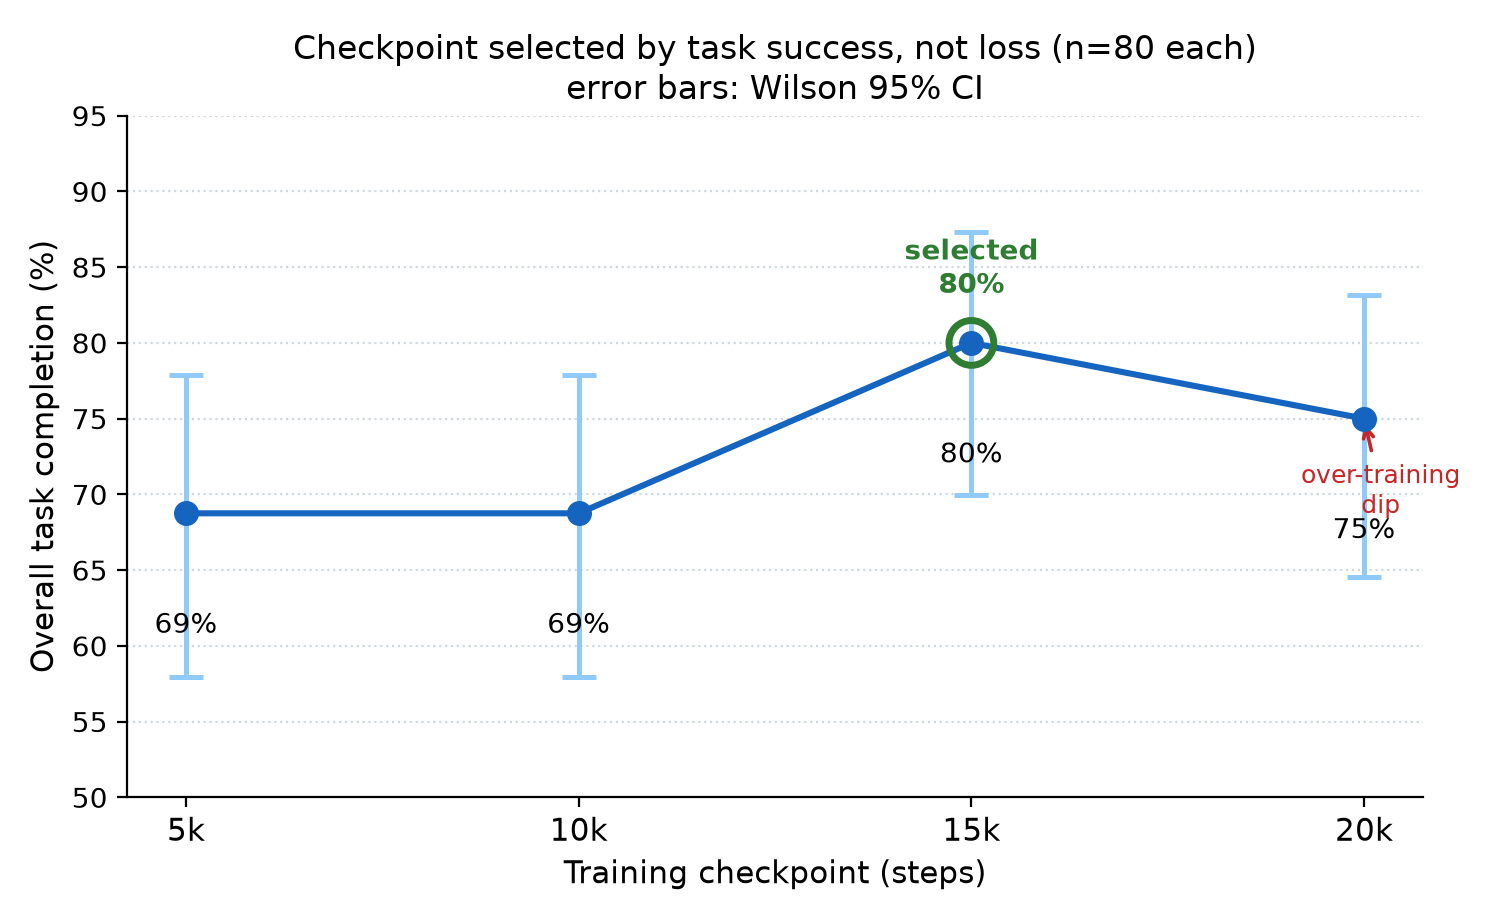
\includegraphics[width=0.8\textwidth,
    alt={A line chart of task-completion rate versus training step, peaking at the 15k checkpoint (80 percent) and dipping at 20k (75 percent), with confidence-interval error bars.}]{figures/checkpoint_selection}
\end{center}
\caption{Task-completion rate versus training checkpoint, selected by closed-loop
success rather than loss. The 15k checkpoint attains the highest rate; the
differences between checkpoints are not statistically significant at $n=80$
(McNemar, all $p \ge 0.19$), so the error bars should be read as overlapping.}
\label{fig:checkpoints}
\end{figure}

\section{Interpretability: the model's predicted plan}
\label{sec:results-interpret}
Because SmolVLA predicts a chunk of 50 future actions, the model's own plan can be
surfaced at each re-planning step. At the very first frame of an episode --- with
the arm still at its home pose, far from the item --- the predicted gripper channel
already transitions to ``closed'' at approximately step~16. In other words, the
policy has decided \emph{to grasp} before it has reached the object. This readout
is decoded directly from the network's output rather than from any hand-written
heuristic, and provides a small but genuine window into the policy's intention.

This behaviour is consistent with the role of action chunking discussed in
\refsec{sec:bg-vla}: by committing to a temporally extended plan rather than a single
next action, the policy encodes an anticipatory intention --- to grasp --- before the
sensory evidence that the item is within reach. It also makes the placement phase
interpretable: as the gripper approaches the basket, the planned gripper channel
transitions back to ``open'' a fixed number of steps ahead of the physical release,
so the moment of intended release can be read from the plan before it occurs. Beyond
its explanatory value, such a readout is practically useful as a lightweight monitor:
a plan that never intends to close, or intends to release while far from the basket,
flags a likely failure before it happens, without any additional model or label.

This form of interpretability is worth distinguishing from post-hoc explanation
methods that attribute a decision to input features after the fact. Here the ``plan''
is not an approximation or a saliency map but the model's literal output --- the
sequence of actions it will execute unless it re-plans --- so reading it involves no
additional assumptions and no auxiliary model. It is admittedly a narrow window: it
reveals what the policy intends to do, not why it intends to do it, and it does not
expose the visual features driving the decision. Nonetheless, for a safety-relevant
system the ability to read a short-horizon intention directly from the controller is
valuable, and it comes for free from the action-chunking design. In the two-VLA vision
of \refsec{sec:future}, an analogous readout of the navigation policy's planned path
would be a natural and cheap safety monitor around moving people.

\section{End-to-end shopping list}
\label{sec:results-orchestrator}
Finally, an orchestrator sequences single-item picks into a shopping list. The user
selects items from a menu of the available products; the robot collects them in
order, with the basket accumulating items across picks (the scene is reset once at
the start, not between items), and re-attempts an item if it misses. This
demonstrates the intended end-to-end behaviour: a language/menu request in,
collected items out.

A caveat observed empirically is that multi-item completion is lower than the
product of the single-item rates would predict. When the first item is already in
the basket, the scene and basket cameras show a configuration the policy never saw
during training (which always began with an empty basket), and this
out-of-distribution view degrades the subsequent pick --- the far-edge water bottle
being the most sensitive. The first item of a list is therefore always as reliable
as the single-item rates in \reftab{tab:peritem}; later items are somewhat less so.
The menu interface (which constrains the request to the known catalogue) and the
retry-on-miss behaviour mitigate this, but the underlying distribution shift is a
data problem, analysed with its remedy in \refsec{sec:disc-limits}.

Two design choices in the orchestrator are worth noting. First, item selection is
made through a fixed menu of the known products rather than by parsing arbitrary free
text; this is a deliberate reliability decision, since the language competence that
matters for the task is grounding a named item in the scene (which the policy does),
not open-vocabulary parsing (which it was not trained for and which a small brittle
parser would get wrong). Second, between items the arm is returned to its home
configuration --- the same start state used during data collection --- so that each
pick begins in-distribution; the scene, however, is not reset, so previously collected
items genuinely accumulate in the basket. The retry-on-miss policy re-attempts a
dropped item a bounded number of times, which recovers many of the stochastic
single-attempt failures at the cost of additional time. Together these make the
orchestrator a faithful end-to-end demonstration of the intended behaviour while
keeping its failure modes attributable to the underlying policy rather than to the
sequencing layer.

\section{Synthesis}
\label{sec:results-synthesis}
Taken together, the results support three claims. First, a compact VLA is
\emph{deployable} under a hard 12~GB budget and reaches a useful 80\% task-completion
rate on this task (\refsec{sec:results-headline}). Second, the largest gains came
from \emph{methodology rather than scale}: the 0\%-to-80\% improvement
(\refsec{sec:results-diagnosis}) followed from diagnosis and from correcting
observability, data boundaries and the target, not from a larger model; and the
prior pilot showed metric and data fixes dominating model choice
(\refsec{sec:results-journey}). Third, the policy is genuinely
\emph{instruction-following} rather than executing a fixed motion
(\refsec{sec:results-language}), and its behaviour is partly \emph{legible} through
its own predicted plan (\refsec{sec:results-interpret}). The clear separation
between a near-solved grasp phase (92.5\%) and a more variable placement phase
(80\%) localises the remaining difficulty to final-drop precision under a stochastic
policy --- precisely the regime the evaluation protocol was designed to measure
honestly.

Read against the research questions of \refsec{sec:rqs}, the chapter answers each in
turn. RQ1 (feasibility) is answered affirmatively by the 80\% headline under a strict
12~GB budget. RQ2 (model versus methodology) is answered by two independent pieces of
evidence: the pilot, where fixing the metric and the data --- not the model --- moved
real performance from an apparent 80\% to a real 40\% and then upward; and the
supermarket task, where the decisive 0\%-to-80\% gain came from observability and data
fixes rather than scale, and where even checkpoint selection had to be made by task
success rather than loss. RQ3 (grounding) is answered by the controlled
instruction-swap test, in which the reach follows the named item across the shelf. RQ4
(failure structure) is answered by the traced diagnosis, which localised the initial
failure to the terminal placement and corrected it by targeted changes. That all four
questions admit clear, evidence-based answers is itself a result: it is a consequence
of designing the evaluation, from the outset, to make such answers possible rather than
to maximise a single headline number.
